\section{Tutorial Resources}
\label{sec:Resources}

	Below are some top sources guides and tutorials for the Raspberry Pi 
	
	\subsection{Raspberry Pi Tutorials}
	
		\subsubsection*{Raspberry Pi Resources}
	
			\url{https://www.raspberrypi.org/resources/}
			\begin{center}
				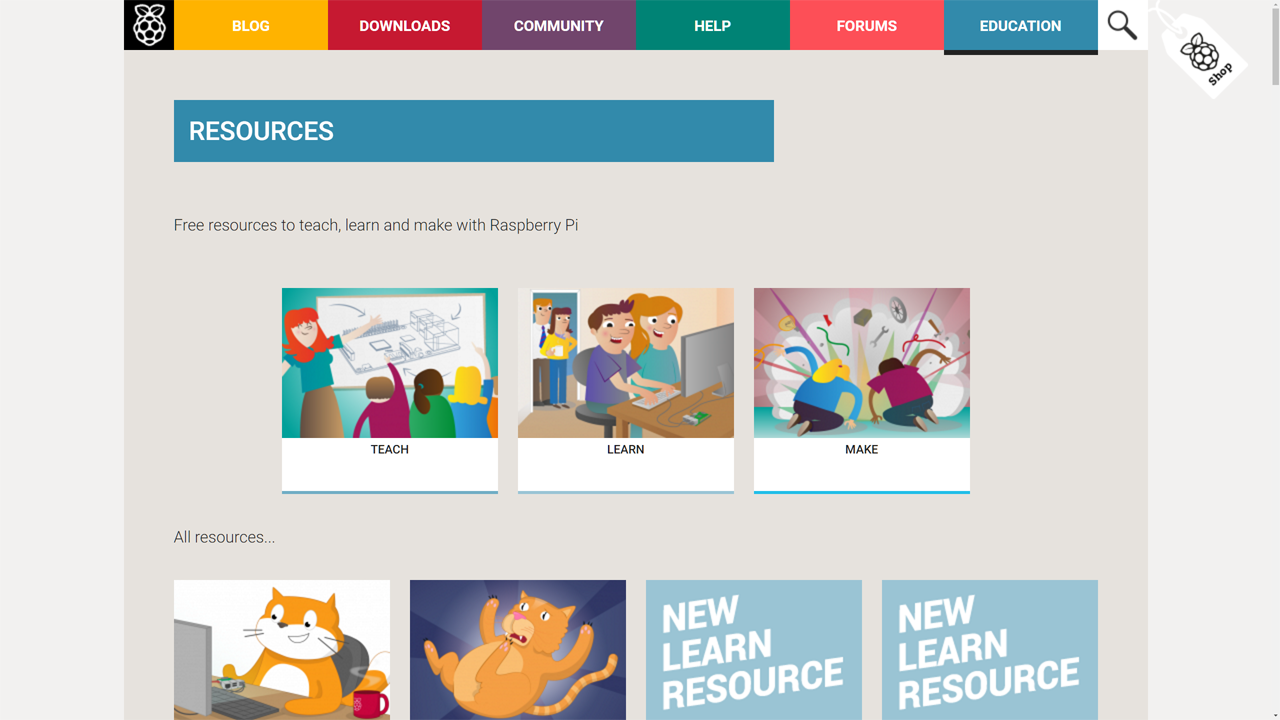
\includegraphics[width=0.5\linewidth]{000_IntroToPi/4_Resources/raspberrypiorg}
			\end{center}

	
			The official Raspberry Pi website should be your first stop, it's chock full of introduction tutorials and project ideas for most of the software we've covered today.
	
		\subsubsection*{The MagPi Magazine}
	
			\url{https://www.raspberrypi.org/magpi/}
			\begin{center}
				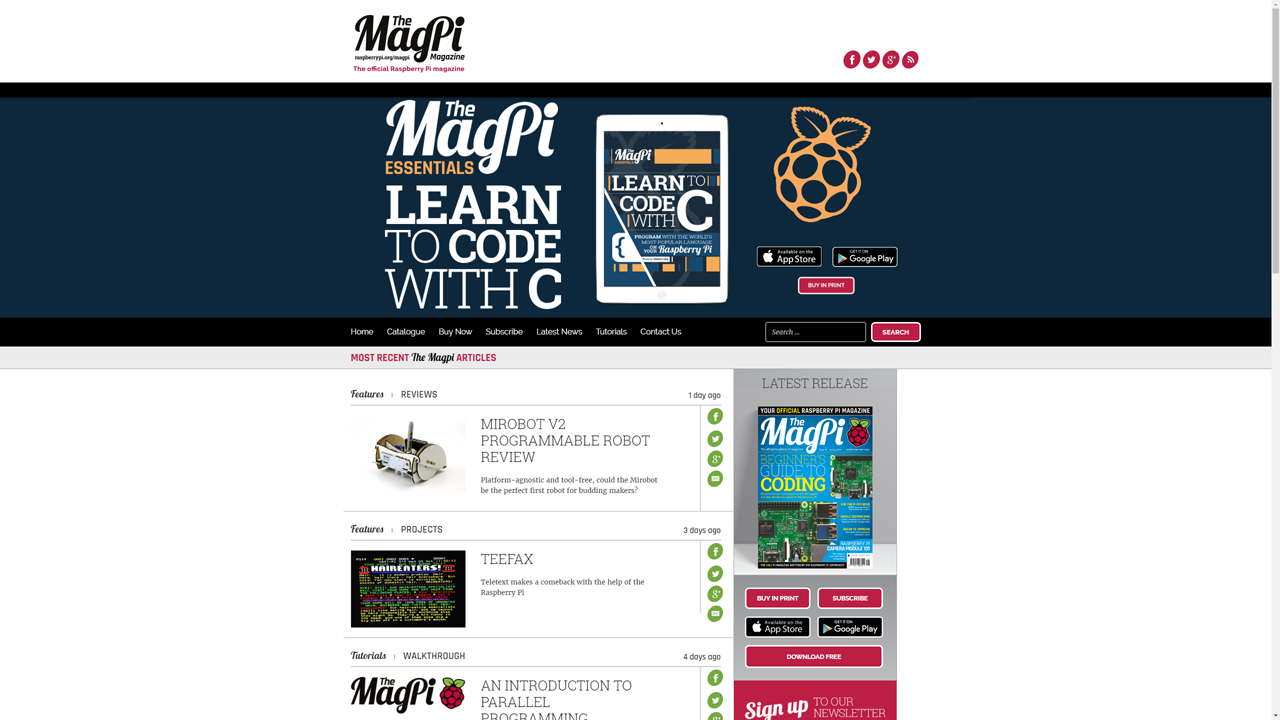
\includegraphics[width=0.5\linewidth]{000_IntroToPi/4_Resources/magpi}
			\end{center}		
				
			The MagPi started as a community run print magazine for the Raspberry Pi, and has now become the official magazine of the Raspberry Pi.
			
			Available in print (can be found in many supermarkets), or as a free download, each one is filled with articles, features and tutorials, all for the Raspberry Pi.
			
		\subsubsection*{The Raspberry Pi Guy}
			
			\url{http://www.theraspberrypiguy.com/tutorials/}
			\begin{center}
				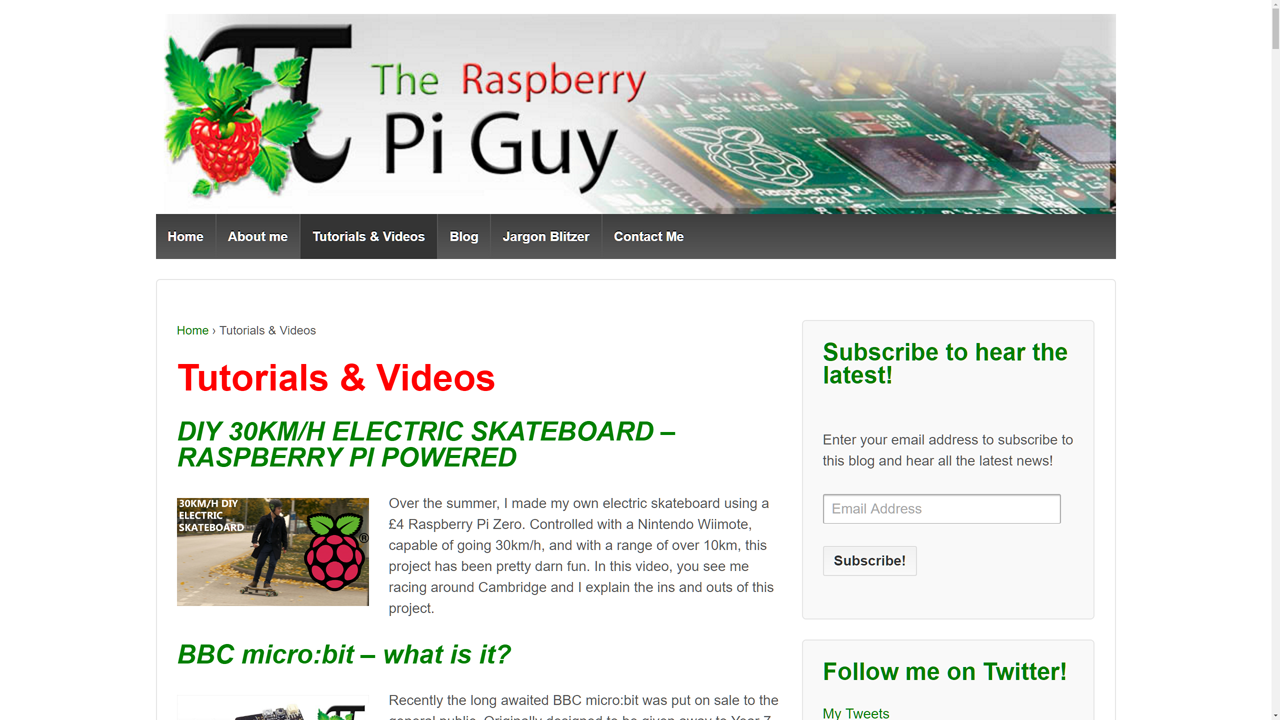
\includegraphics[width=0.5\linewidth]{000_IntroToPi/4_Resources/piguy}
			\end{center}	
			
			Matt was one of the first people to start producing regular video content for the Raspberry Pi, he was only 12 when the Pi was first released!
			
			Every few months, he produces a new video tutorial, showing off cool projects and uses for the Raspberry Pi, covering things as wide as Steam game streaming, robotics, or even building an electric skateboard.
		
	\subsection{Programming Language Tutorials}
	
		Ready to stretch your legs and try another programming language? Here are some places to look for quality programming language tutorials
		
		\subsection*{Codeacademy}
		
		\url{https://www.codecademy.com/}
		
		Codeacademy has tutorials for a large number of languages, we'd recommend \textbf{Java} for a great second language and introduction to object orientated programming, or \textbf{Javascript} if you'd like to learn some programming for web purposes.
		
		\footnotesize \textit{Confusingly, Java and Javascript are entirely seperate languages.} \normalsize
	
		\subsection*{C and C++}
		
		\url{http://www.learn-c.org/}
		\\ \url{http://www.learncpp.com/}
		
		If you're feeling brave, C and C++ are traditional programming languages that are widely used today. C++ was designed to follow on from C, so it makes sense to start there.